% if you want the answers to appear uncomment the below
\documentclass[answers]{exam}
% otherwise uncomment the below
% \documentclass{exam}
\usepackage[bottom]{footmisc}
\usepackage{graphicx}
\usepackage[letterpaper, margin=.9in]{geometry}
\usepackage{natbib}
\bibpunct{(}{)}{;}{a}{,}{,}
\usepackage{url}
\def\UrlFont{\rm}


\usepackage{Sweave}

\usepackage[utf8x]{inputenc}
\usepackage{array}
\usepackage{verbatim}
\usepackage{amsfonts}
\usepackage{amsmath}
%\usepackage{lineno}
\setlength{\parskip}{2ex} 
%\setlength{\parindent}{0ex}

% Cannot place floats in figure environment.
\usepackage{caption}
\usepackage{newfloat}
%\DeclareCaptionListFormat{myliststyle}{#1.#2}
\DeclareCaptionType{mytype}[Solution Fig.][List of mytype]
\newenvironment{myfigure}{\captionsetup{type=mytype}}{}



\newenvironment{packed_enum}{
\begin{enumerate}
 \setlength{\itemsep}{0pt}
  \setlength{\parskip}{0pt}
  \setlength{\parsep}{0pt}
}{\end{enumerate}}
\newenvironment{packed_item}{
\begin{itemize}
 \setlength{\itemsep}{0pt}
  \setlength{\parskip}{0pt}
  \setlength{\parsep}{0pt}
}{\end{itemize}}

 \newcommand\independent{\protect\mathpalette{\protect\independenT}{\perp}}
    \def\independenT#1#2{\mathrel{\setbox0\hbox{$#1#2$}%
    \copy0\kern-\wd0\mkern4mu\box0}} 


\bibliographystyle{plainnat}

\pagestyle{myheadings}
\markright{Advanced Topics in Causal Inference \hfill  R Lab \#4 \hfill}


\title{R Lab 4 - Estimation, Part I: IPTW}
\author{Advanced Topics in Causal Inference}
\date{}

\begin{document}
\maketitle

\Sconcordance{concordance:RLab4_answers.tex:RLab4_answers.Rnw:%
1 260 1 1 2 4 0 1 2 13 1 1 2 4 0 1 2 26 1 1 6 5 0 1 4 5 0 1 7 5 0 1 1 3 %
0 1 5 3 0 1 1 1 4 2 0 1 1 3 0 1 2 1 4 9 0 1 1 6 0 2 1 3 0 1 9 11 1 1 3 %
5 0 1 2 1 4 6 0 1 10 11 0 1 2 1 4 8 0 1 1 3 0 1 4 9 0 1 7 11 1 1 3 2 0 %
1 1 5 0 1 4 8 0 1 2 1 3 2 0 1 1 5 0 1 4 8 0 1 2 23 1 1 2 4 0 1 2 12 1 1 %
4 3 0 1 3 4 0 1 4 2 0 1 2 4 0 1 34 35 0 1 5 10 0 1 4 9 0 1 5 10 0 1 2 2 %
1 1 4 49 1 1 2 1 0 1 3 4 0 1 2 6 1 1 2 4 0 1 2 21 1 1 2 4 0 1 2 27 1 1 %
2 4 0 1 2 8 1 1 13 15 0 1 2 11 1 1 6 5 0 1 4 5 0 1 7 5 0 3 1 3 0 1 6 4 %
0 3 1 3 0 1 5 14 0 4 1 3 0 1 11 10 1 1 6 8 0 1 7 5 0 1 3 4 0 1 4 2 0 2 %
1 3 0 1 5 9 0 1 1 6 0 1 1 6 0 1 1 6 0 4 1 3 0 1 11 10 1 1 6 5 0 1 1 3 0 %
1 4 5 0 1 4 8 0 1 1 3 0 1 7 8 1 1 4 9 0 1 2 4 0 1 7 9 1 1 4 9 0 1 2 4 0 %
1 7 10 1 1 4 3 0 1 1 6 0 1 2 1 1 1 4 3 0 1 1 6 0 1 2 4 1 1 3 5 0 1 4 2 %
0 2 1 6 0 1 2 9 1 1 3 5 0 1 5 6 0 1 17 18 0 1 4 5 0 1 3 7 0 1 1 3 0 1 2 %
1 3 2 0 2 1 6 0 1 2 28 1 1 2 1 0 1 1 3 0 1 2 12 1 1 4 3 0 1 3 4 0 1 4 2 %
0 1 2 4 0 1 69 70 0 1 5 9 0 1 2 6 0 1 1 6 0 1 4 9 0 1 5 9 0 1 2 6 0 1 1 %
6 0 1 2 43 1}


\noindent \textbf{Assigned:} October 5, 2021\\
\textbf{Lab due:} October 12, 2021 on bCourses. Please answer all questions and include relevant \texttt{R} code. You are encouraged to discuss the assignment in groups, but should not copy code or interpretations verbatim. Upload your own completed lab to bCourses.

\noindent \textbf{Last lab:} \\
Make explicit assumptions sufficient for identifiability, and under those assumptions, write the target causal parameter as a statistical parameter.


\noindent \textbf{This lab:}\\
1. IPTW estimation for simple treatment specific means. \\
2. IPTW estimation for working marginal structure models. \\
3. Evaluate performance of IPTW estimators. \\

\noindent \textbf{Next lab:}\\
Introduction to the \texttt{ltmle} package.



\begin{center}
\noindent\rule{18cm}{0.4pt}
\end{center}


\section{Introduction and Motivation}

Last lab we derived statistical parameters (functions of the observed data distribution, $P_0$) that, under certain assumptions, are equal to our target causal parameters (functions of the counterfactual distribution, $P_{U,X}$) of interest. These statistical parameters are also called \textit{estimands}; specifically, in the last lab we derived g-computation estimands. In this lab, we will introduce another statistical parameter: the IPTW estimand. It turns out that g-computation and IPTW estimands are equivalent! %We could estimate the g-computation estimand directly via the g-computation \textit{estimator} (coming up in a later lab!), or we could use another method: the IPTW estimator. 

\subsection{Showing the g-computation and IPTW estimands are equivalent}

Suppose we have $t=1,2$ timepoints, no censoring, and we want to estimate the causal parameter $E[Y_{\bar{a}(2)^*}]$.


\begin{align}
\intertext{Under sequential randomization and positivity, the corresponding IPTW estimand is equal to:} 
\Psi(P_0)  = & E_0\Big[ \frac{\mathbb{I}[\bar{A}(2) = \bar{a}(2)^*]}{g_0(A(1)|L(1))g_0(A(2)|\bar{L}(2), A(1))}Y\Big] \label{eq1}
\intertext{Using the definition of expectations, (e.g., $E[X] = \sum_xxP(X=x)$) equation (\ref{eq1}) can be rewritten as:}
 = &\sum_{y, \bar{a}(2), \bar{l}(2)} y \nonumber\\
 & \times P_0(Y = y, \bar{A}(2) = \bar{a}(2), \bar{L}(2) = \bar{l}(2)) \nonumber\\
 & \times \frac{\mathbb{I}[\bar{A}(2) = \bar{a}(2)^*]}{g_0(A(1) = a(1)| L(1) = l(1))g_0(A(2) = a(2)|\bar{L}(2) = \bar{l}(2), A(1) = a(1))} \label{eq2}
\intertext{Factorize $P_0(Y = y, \bar{A}(2) = \bar{a}(2), \bar{L}(2) = \bar{l}(2))$ and re-write equation (\ref{eq2}) as: }
= & \sum_{y, \bar{l}(2)} y \nonumber\\
& \times P_0(Y = y| \bar{A}(2) = \bar{a}(2)^*, \bar{L}(2) = \bar{l}(2)) \nonumber\\
& \times P_0(A(2) = a(2)^* | \bar{L}(2) = \bar{l}(2), A(1) = a(1)^*)\nonumber\\
& \times P_0(L(2) = l(2) | A(1) = a(1)^*, L(1) = l(1))  \nonumber\\
& \times P_0(A(1) = a(1)^* | L(1) = l(1)) \nonumber\\
& \times P_0(L(1) = l(1)) \nonumber\\
& \times \frac{1}{g_0(A(1) = a(1)^*| L(1) = l(1))g_0(A(2) = a(2)^*|\bar{L}(2) = \bar{l}(2), A(1) = a(1)^*)} \label{eq3}\\
\intertext{Canceling out terms (remember that $P_0(A|L) = g_0(A|L)$), we can rewrite equation (\ref{eq3}) as:}
= & \sum_{y, \bar{l}(2)} y   \nonumber\\
& \times P_0(Y = y| \bar{A}(2) = \bar{a}(2)^*, \bar{L}(2) = \bar{l}(2)) \nonumber\\
& \times P_0(L(2) = l(2) | A(1) = a(1)^*, L(1) = l(1))  \nonumber\\
& \times P_0(L(1) = l(1)) \\
\intertext{Again, by the definition of expectations:}
= & \sum_{\bar{l}(2)} E[ Y | \bar{A}(2) = a(2)^*, \bar{L}(2) = \bar{l}(2)]  \nonumber\\
& \times P_0(L(2) = l(2) | A(1) = a(1)^*, L(1) = l(1)) \nonumber\\
& \times P_0(L(1) = l(1))\label{lasteq}
\end{align}
The last equation (\ref{lasteq}) is exactly the longitudinal g-computation formula! (Recall that we derived this g-computation estimand in \texttt{R} Lab 3).

\subsection{Estimation using IPTW and modified IPTW}

Now onto estimation! 

\noindent In previous labs, we had been dealing with distributions (e.g., $P_0$) and values of functions of these distributions (e.g., $\Psi(P_0)$, or statistical estimands) that are often unknown to us when dealing with applied data. Now, we are handed a dataset -- a \textit{finite} sample of $n$ i.i.d. observations of $O$, which follows the empirical distribution, $P_n$. $P_n$ puts weight $\frac{1}{n}$ on each observation, $O_i$, $i = 1,...,n$. Using a function of the finite sample drawn from $P_n$, we aim to estimate our statistical estimands.

\noindent Recall that the IPTW \textit{estimand} is the following (note this is equation (\ref{eq1}) above, extended to $K$ timepoints): 

$$\Psi(P_0) =E\Bigg[\frac{\mathbb{I}[\bar{A}(K)=\bar{a}(K)]}{\prod_{t=1}^Kg_0(A(t)|\bar{A}(t-1), \bar{L}(t))}Y\Bigg]$$

\noindent where ${g_0(A(t)|\bar{A}(t-1), \bar{L}(t))}$ is the product of time-point-specific predicted probabilities of observed treatment and/or censoring, given observed treatment and covariate history. 

The \textbf{IPTW \textit{estimator}} (that is aimed at estimating the IPTW estimand) applied to our empirical data is then:

\begin{align*}
\hat{\Psi}(P_n) & =\frac{1}{n}\sum_{i=1}^n\frac{\mathbb{I}[\bar{A}_i(K)=\bar{a}_i(K)]}{\prod_{t=1}^Kg_n(A_i(t)|\bar{A}_i(t-1), \bar{L}_i(t))}Y_i \\
& =\frac{1}{n}\sum_{i=1}^n\mathbb{I}[\bar{A}_i(K)=a_i(K)]\hat{w}_iY_i \\
& \intertext{where $\hat{w}_i = \frac{1}{g_n(A_i(t)|\bar{A}_i(t-1), \bar{L}_i(t))}$ (i.e., the IPTW weights).}
\end{align*}

We will also implement a modified version of the IPTW estimator, called the \textbf{modified Horvitz-Thompson estimator}: 

\begin{align*}
\hat{\Psi}(P_n) & =\frac{\sum_{i=1}^n \frac{\mathbb{I}[\bar{A}_i = \bar{a}]}{\prod_{t=1}^Kg_n(A_i(t)|\bar{L}_i(t), \bar{A}_i(t-1))}Y_i}{\sum_{i = 1}^n \frac{\mathbb{I}[\bar{A}_i = \bar{a}]}{\prod_{t=1}^Kg_n(A_i(t)|\bar{L}_i(t), \bar{A}_i(t-1))}}\\
& =\frac{\sum_{i=1}^n\mathbb{I}[\bar{A}_i(K)=\bar{a}_i(K)]\hat{w}_iY_i}{\sum_{i=1}^n\mathbb{I}[\bar{A}_i(K) = \bar{a}_i(K)]\hat{w}_i} \\
\end{align*}

\noindent This is essentially the standard IPTW estimator, but we divide by the sample average of the weights. The advantage to the Horvitz-Thompson estimator is that it 1) may reduce the variability of the IPTW estimates and 2) respects the parameter space (for example, if $Y$ is binary, we will ensure that we don't get an expectation less than 0 or greater than 1).

\subsection{Using IPTW weights to estimate MSM parameters}

Let $m(\bar{a}|\beta)$ be a (working) model for $E[Y_{\bar{a}}]$. For example, our working MSM could be:

\[
m(\bar{a}|\beta) =\beta_0+\beta_1\sum_{t=1}^Ka(t)
\] 

\noindent Then, if we either assume the MSM is correctly specified or if we choose $g^*(\bar{A})=1$ as the projection function, then our target causal parameter is:
\[
\Psi^F(P_{U,X})=\arg\min_\beta \sum_{\bar{a} \in \mathcal{A}}(Y_{\bar{a}}-m(\bar{a}|\beta))^2
\]

\noindent We can estimate this parameter (the $\beta$s) using a weighted regression with unstabilized weights (which are just the weights, $\hat{w}_i$, above):

\[
\hat{w}_i = \frac{1}{\prod_{t=1}^Kg_n(A_i(t)|\bar{A}_i(t-1), \bar{L}_i(t))}
\]

\noindent We could alternatively define our target parameter value $\beta$ using a different projection function. For example, a common choice is $g(\bar{A})$, defined as the marginal probability of regime $\bar{A}$ occurring. Now the target causal parameter is defined as:

\[
\Psi^F(P_{U,X})=\arg\min_\beta \sum_{\bar{a} \in {\cal A}}(Y_{\bar{a}}-m(\bar{a}|\beta))^2 g(\bar{A})
\]

\noindent If the MSM is correctly specified, the choice of projection function $g(\bar{A})$ will not change the value of $\beta$ that minimizes the sum of the squared residuals (and therefore will not change the true value of the target causal parameter). However, if the MSM is not correctly specified, the choice of projection function will result in a different true value of the target causal parameter -- one that puts more weight on the treatment regimes with more representation in the data.

\noindent For this second target parameter, an IPTW estimator of $\beta$ can be implemented using the following stabilized weights:

\[
\hat{sw}_i = \frac{g_n(\bar{A}_i(K))}{\prod_{t=1}^Kg_n(A_i(t)|\bar{A}_i(t-1), \bar{L}_i(t))}
\]

\noindent The numerator, $g_n(\bar{A}_i(K))$, is the marginal probability of seeing the subject's particular treatment regime. Informally, the advantage to using stabilized weights is that it prevents rare exposure histories from being assigned large weights.


\begin{figure}
\begin{center}

\includegraphics[width=.35\textwidth]{IPTWpic.png}
\caption{Inverse weighting.}
\end{center}
\end{figure}

\section{This lab}

Finally, your GSR gives you some data! One-thousand students were sampled from the school, which we can treat as 1,000 i.i.d. copies of $O$.

\noindent This lab will walk you through loading your GSR data, estimating (using IPTW) the parameters that inform us about the effects of sleep, and evaluating how well IPTW works. IPTW performance will be measured by evaluating the estimator's bias (or, the expected difference between the point estimate, $\psi_n$, and the true parameter value):

\[
Bias(\hat{\Psi}(P_n)) = E_0[\hat{\Psi}(P_n) - \Psi(P_0)]
\]

\noindent the estimator's variance (or, the average squared difference between each estimate and the average of the estimates):

\[
Variance(\hat{\Psi}(P_n)) = E_0\Bigg[\Big[\hat{\Psi}(P_n) - E_0[\hat{\Psi}(P_n)]\Big]^2\Bigg]
\]

\noindent and the estimator's mean-squared error (MSE, or, the average squared distance the estimator is from the true parameter value):
\[
E_0\Big[[\hat{\Psi}(P_n) - \Psi(P_0)]^2\Big] = Bias^2 + Variance
\]

For this lab, you'll answer questions for two of the data generating systems we've been working with in previous labs. We are now on step 6 (estimation) of the causal roadmap. See \texttt{R} Lab 1 for specifying the causal model (step 1), \texttt{R} Lab 2 for the causal questions and parameters of interest (step 2), \texttt{R} Lab 1 and 2 for the link between the SCM and observed data (step 3), and \texttt{R} Lab 3 for identifiability and specification of the target parameter of the observed data distribution (step 4 and 5, respectively).


\subsection{To turn in:}


\noindent\fbox{
    \parbox{\textwidth}{

\textbf{\underline{For each of the 2 data structures listed below, answer the following questions:}} \\



\begin{enumerate}
\item \textbf{Implement IPTW for estimation} of statistical parameters that, under sequential randomization and positivity assumptions, are equal to our causal parameters of interest:
\begin{itemize}
\item[-] For both data structures, implement IPTW for estimation of treatment specific means. Implement both the \textbf{standard IPTW} and \textbf{modified Horvitz-Thompson IPTW} estimators.
\item[-] For Data Structure 2 ONLY, implement IPTW to estimate the parameters of an MSM using an \textbf{MSM with unstabilized weights}. As a bonus, you may additionally estimate the parameters of an MSM with stabilized weights. (Fall 2020 -- not required)
\end{itemize}
Within the IPTW estimation process, \textbf{comment on the distributions of the predicted probabilities and weights} that went into the IPTW estimates. Also, \textbf{interpret each IPTW estimate.}
\item \textbf{Compare performance metrics of each of the estimators}. Specifically, evaluate the bias, variance, and mean-squared error (MSE) of each of the estimators.
\end{enumerate}
    
    }
}

\pagebreak
\noindent\large\textbf{Data Structure 0: $O = (L(1), A(1), L(2), A(2), Y)$}
\normalsize

\noindent \underline{Target parameter:} we are interested in the expected $Y$ if everyone got treatment regime $\bar{a}(2) = 1$.
\[
\Psi^F(P_{U,X}) = E_{U,X}[Y_{\bar{a}(2)=1}]
\]

\begin{enumerate}
\item \textbf{IPTW for estimation:}
\begin{enumerate}
\item Load \texttt{DataStructure0.RData} using the \texttt{load()} function. Make sure you have specified the correct file path. You should see 3 new things come up in your global environment:
\begin{packed_item}
\item[-] \texttt{ObsData0} -- this the data given to you by your GSR. It is a dataframe of 1,000 observations (note: it follows Data Structure 0 from the previous lab).
\item[-] \texttt{Psi.F0} -- this is the true $\Psi^F(P_{U,X})$ value for the target causal parameter $E_{U,X}[Y_{\bar{a}(2)=1}]$ (generated in lab 3).
\item[-] \texttt{generate\_data0} -- this is the function that generates $n$ copies of Data Structure 0.
\item[-] \texttt{generate\_data0\_intervene} -- we won't use this function in this lab, so if you'd like you can remove it from your global environment using the \texttt{rm()} function.
\begin{Schunk}
\begin{Sinput}
> rm(generate_data0_intervene)
\end{Sinput}
\end{Schunk}
\end{packed_item}
\item Assign the number of students to \texttt{n}.
\item Estimate the IPTW weights:
\begin{enumerate}
\item Estimate the probability of receiving treatment $P_0(A(t)=1|\bar{L}(t), \bar{A}(t-1)) = g_0(A(t)=1|\bar{L}(t), \bar{A}(t-1))$ for $t = 1,2$ using correctly specified parametric regression models. The correct model specifications are (optional: refer back to \texttt{R} lab 3 to verify!):
\begin{align*}
g_0(A(1)=1|L(1)) & = expit[\beta_0 + \beta_1L(1)] \\
g_0(A(2)=1|\bar{L}(2), A(1)) & = expit[\beta_0 + \beta_1L(1) + \beta_2A(1) + \beta_3L(2)]
\end{align*}
Use the \texttt{glm()} function, and specify the arguments \texttt{family = `binomial'} for logistic regression and \texttt{data = ObsData0} to call the correct dataset. 
\item Predict each subject's probability of the exposure at time $t$, given his or her observed exposure and covariate history, i.e., $g_n(A_i(t)=1|\bar{A}_i(t-1), \bar{L}_i(t))$. Name these vectors \texttt{gA1.1} and \texttt{gA2.1}. Also evaluate each subject's probability of the observed exposure at time $t$, given their observed exposure and covariate history, i.e., $g_n(A_i(t)|\bar{A}_i(t-1), \bar{L}_i(t))$. Name these vectors \texttt{gA1} and \texttt{gA2}.\\
\textit{Hint:} use the \texttt{predict()} function on each of the logistic regressions applied above, specifying \texttt{type = `response'} as an argument.
\item \textbf{Look at the distributions of the predicted probabilities of exposure using the \texttt{hist()} and \texttt{summary()} functions. What are we able to assess by looking at the distribution of the predicted probabilities of exposure? Any cause for concern here?}
\item Obtain the indicator variable $\mathbb{I}[\bar{A}_i(2)=1]$ by creating a logical variable that indicates which students had a treatment history $\bar{a}(2) = 1$:
\begin{Schunk}
\begin{Sinput}
> I11 = ObsData0$A1 == 1 & ObsData0$A2 == 1
\end{Sinput}
\end{Schunk}
\item Calculate the weights $\hat{w}_i$ by taking the inverse of the product of the time point specific predicted probabilities of the observed treatment, i.e.: 

\[
\hat{w}_i = \frac{1}{g_n(A_i(1)|L_i(1))\times g_n(A_i(2)|A_i(1), L_i(1), L_i(2))}
\]

Do this \textit{only for people who got treatment history $\bar{a} = 1$} by using the indicator variable you created in the previous step. \textbf{Look at the distribution of these weights. What can we assess by looking at the distribution of the estimated weights? Any cause for concern here?\\
\textit{Bonus}: what are the drawbacks of only using this method of assessment, as opposed to looking at the propensity scores (as in step two steps ago)?}
\end{enumerate}
\item Implement the \textbf{standard IPTW estimator} by taking the empirical mean of the weighted outcomes:
\begin{align*}
\hat{\Psi}(P_n) & =\frac{1}{n}\sum_{i=1}^n\frac{\mathbb{I}[\bar{A}_i(2)=1]}{g_n(A_i(1)|L_i(1))\times g_n(A_i(2)|A_i(1), L_i(1), L_i(2))}Y_i \\
& =\frac{1}{n}\sum_{i=1}^n\underbrace{\mathbb{I}[\bar{A}_i(2)=1]}_{\textit{You obtained this in step iv!}} \times \underbrace{\hat{w}_i}_{\textit{You obtained this in step v!}} \times \underbrace{Y_i}_{\textit{This is the outcome variable in the data!}}
\end{align*}
\item Implement the \textbf{modified Horvitz-Thompson estimator}:
\begin{align*}
& = \frac{\frac{1}{n}\sum_{i=1}^n\mathbb{I}[\bar{A}(2)_i=1]\hat{w}_iY_i}{\frac{1}{n}\sum_{i=1}^n\mathbb{I}[\bar{A}(2)_i=1]\hat{w}_i}
\end{align*}

where, again, $\hat{w}_i = \frac{1}{g_n(A_i(1)|L_i(1))\times g_n(A_i(2)|A_i(1), L_i(1), L_i(2))}$. \\
\textit{Hint: Divide the result from the previous step by the average of the IPTW weights!}
\item \textbf{Interpret your results.}
\end{enumerate}

\begin{solution}


\begin{Schunk}
\begin{Sinput}
> # load the data, functions, and objects associated with ObsData0.
> load("DataStructure0.RData")
\end{Sinput}
\end{Schunk}
\begin{Schunk}
\begin{Sinput}
> # assign the number of students to n
> n = nrow(ObsData0)
\end{Sinput}
\end{Schunk}
\begin{Schunk}
\begin{Sinput}
> ### IPTW estimation - Data 0###
> 
> # estimate treatment mechanism g(A(t)=1|Lbar(t), Abar(t-1)) = P(A(t)=1|Lbar(t), Abar(t-1))
> # using correctly specified logistic regression
> gA1.reg = glm(A1 ~ L1, family = "binomial", data = ObsData0)
> gA2.reg = glm(A2 ~ L1 + A1 +  L2, family = "binomial", data = ObsData0)
\end{Sinput}
\end{Schunk}
\begin{Schunk}
\begin{Sinput}
> # predict the probability of having A(t) = 1 at time t, given the observed history
> # g(A(t) = 1|Lbar(t), Abar(t-1)) = P(A(t) = 1|Lbar(t), Abar(t-1))
> gA1.1 = predict(gA1.reg, type = "response")
> gA2.1 = predict(gA2.reg, type = "response")
> # predict the probability of observed exposure at time t, given observed history
> # g(A(t) | Lbar(t), Abar(t-1)) = P(A(t)|Lbar(t), Abar(t-1))
> gA1 = ifelse(ObsData0$A1 == 1, gA1.1, 1-gA1.1)
> gA2 = ifelse(ObsData0$A2 == 1, gA2.1, 1-gA2.1)
\end{Sinput}
\end{Schunk}

\begin{Schunk}
\begin{Sinput}
> # distribution of probability of having A(t) = 1 at time t, given the observed history
> # for t = 1, 2
> summary(gA1.1)
\end{Sinput}
\begin{Soutput}
   Min. 1st Qu.  Median    Mean 3rd Qu.    Max. 
 0.3340  0.3340  0.5753  0.4590  0.5753  0.5753 
\end{Soutput}
\begin{Sinput}
> summary(gA2.1)
\end{Sinput}
\begin{Soutput}
   Min. 1st Qu.  Median    Mean 3rd Qu.    Max. 
 0.4471  0.5188  0.6838  0.6720  0.8495  0.8827 
\end{Soutput}
\begin{Sinput}
> hist(gA1.1, main = "Prob A1 is 1, given past variables", xlim = c(0,1))
> hist(gA2.1, main = "Prob A2 is 1, given past variables", xlim = c(0,1))
\end{Sinput}
\end{Schunk}
\begin{myfigure}
\begin{center}
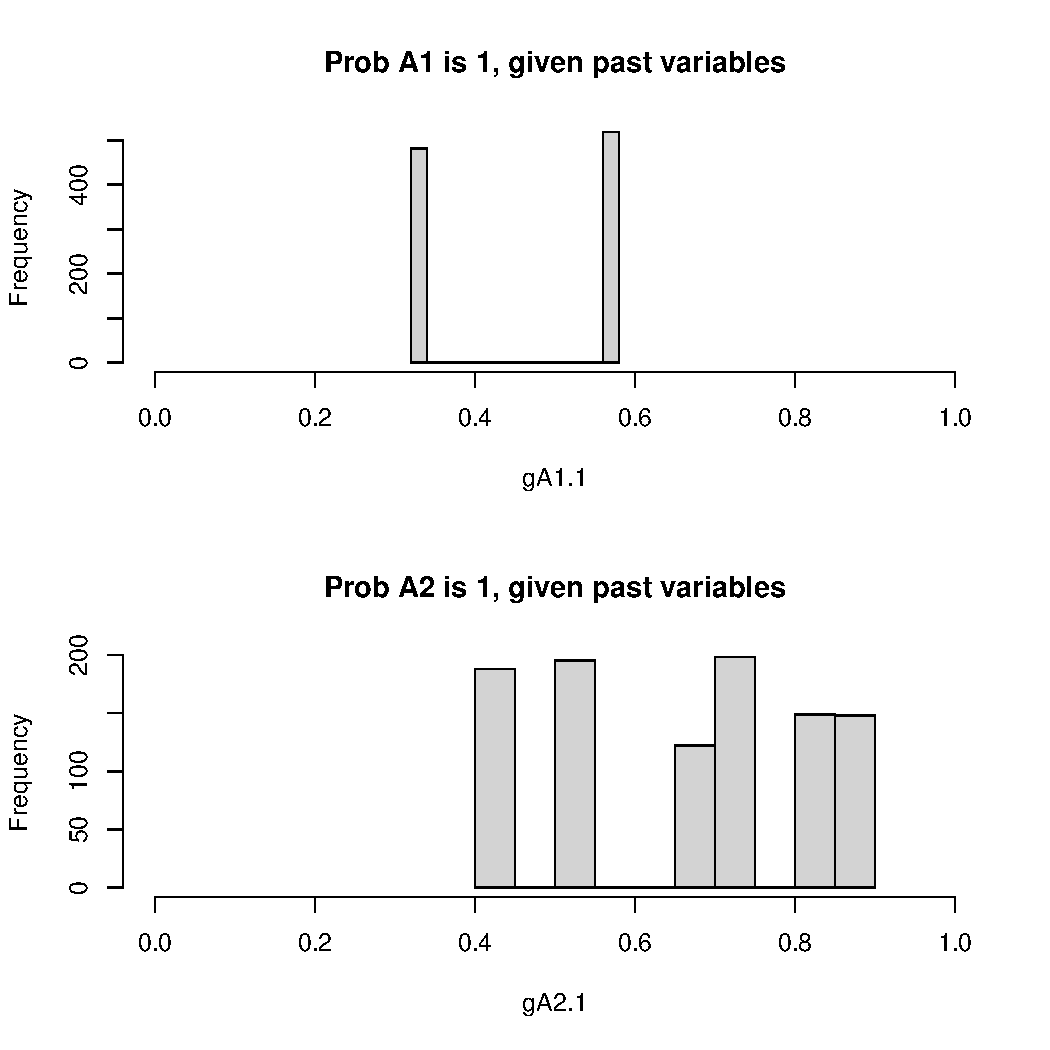
\includegraphics[width=.4\textwidth]{g1Hist0.pdf}
\caption{Plot histograms of $g_n(A(t) = 1|\bar{L}(t), \bar{A}(t-1))$.}
\label{Fig:g1Hist0}
\end{center}
\end{myfigure}

Looking at the distribution of the estimated conditional probabilities of exposure (or propensity scores) is a good way to diagnose practical positivity violations. Based on the summary statistics and histograms, the distribution of the propensity scores are mostly away from 0 and 1. Therefore, there's no indication of near positivity violations.



\begin{Schunk}
\begin{Sinput}
> # indicator variables to identify subjects with abar(2) = 1 
> I11 = ObsData0$A1 == 1 & ObsData0$A2 == 1 
\end{Sinput}
\end{Schunk}

\begin{Schunk}
\begin{Sinput}
> # each subject gets a weight inverse to the product of the predicted probabilities of 
> # observed exposure, given past exposure
> w = 1/(gA1*gA2)
\end{Sinput}
\end{Schunk}
\begin{Schunk}
\begin{Sinput}
> # alternative implementation: note that we will multiply these weights by an 
> # indicator variable that indicates which students had treatment history 
> # abar(2)=1, so we could instead calculate the weights as the product of 
> # the probability of exposure at t=1 and t=2 
> #
> # weights associated with observations that do not have treatment abar(2)=1
> # will be multiplied by zero, so these two implementations are equivalent
> w.alt = 1/(gA1.1 * gA2.1)
\end{Sinput}
\end{Schunk}

\begin{Schunk}
\begin{Sinput}
> # look at the distribution of the weights for people who got abar(2) = 1 
> summary(w[I11])
\end{Sinput}
\begin{Soutput}
   Min. 1st Qu.  Median    Mean 3rd Qu.    Max. 
  2.542   2.788   3.524   3.409   3.888   4.412 
\end{Soutput}
\begin{Sinput}
> hist(w[I11], main = "Distribution of weights \n for people with treatment history = 1")
\end{Sinput}
\end{Schunk}
\begin{Schunk}
\begin{Sinput}
> # alternative implementation: distribution of weights for people who got abar(2)=1
> summary(w.alt[I11]) # note: same as above
\end{Sinput}
\begin{Soutput}
   Min. 1st Qu.  Median    Mean 3rd Qu.    Max. 
  2.542   2.788   3.524   3.409   3.888   4.412 
\end{Soutput}
\end{Schunk}
\begin{myfigure}
\begin{center}
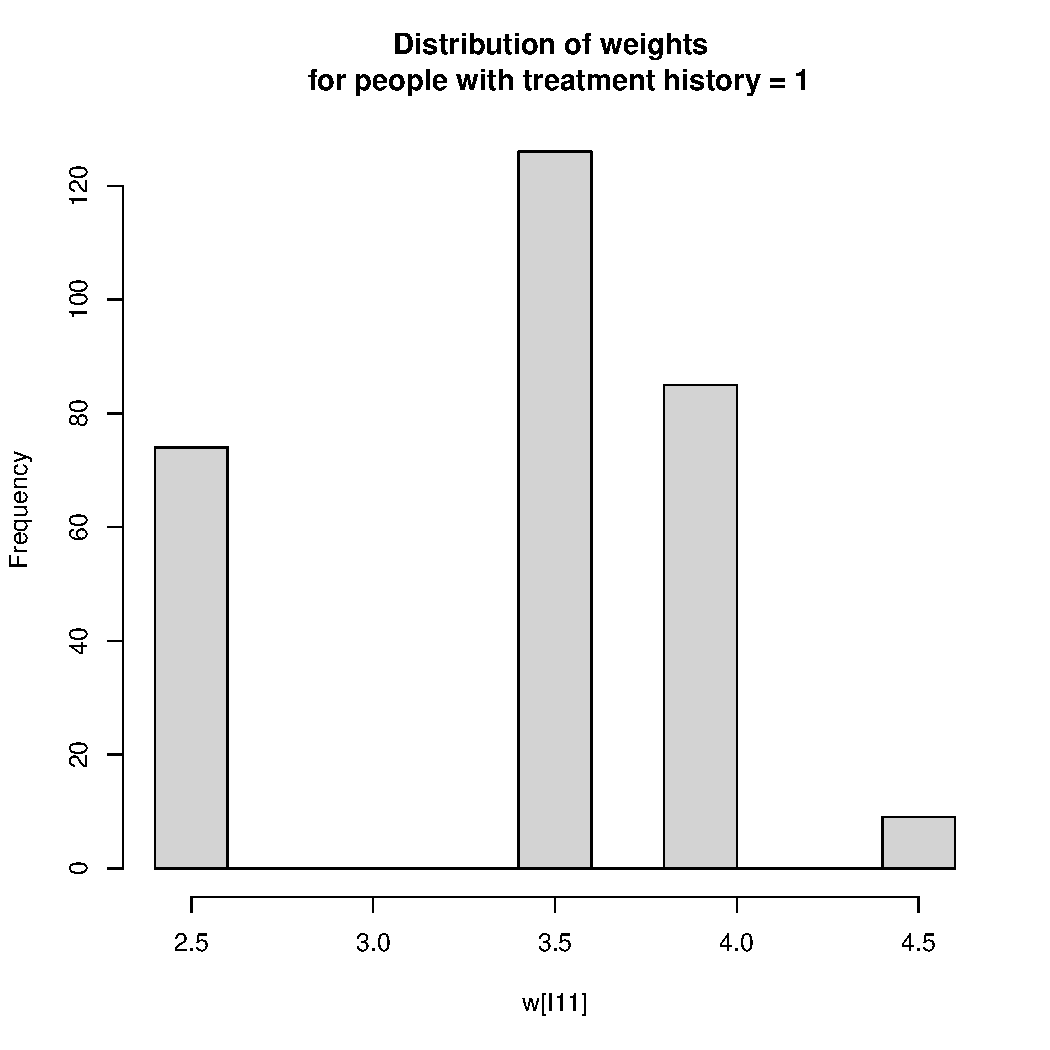
\includegraphics[width=.4\textwidth]{w11Hist0.pdf}
\caption{Distribution of the weights, $w_i = \frac{1}{\prod_{t=1}^Kg_n(A_i(t)|\bar{L}_i(t), \bar{A}_i(t-1))}$}
\label{Fig:w11Hist0}
\end{center}
\end{myfigure}

Again, looking at the distribution of the estimated IPTW weights can assess positivity violations (where extreme weights are a sign of near positivity violations). The drawback of only using the distribution of the weights as a method for diagnosing positivity is that the absence of extreme weights does not guarantee that there are no positivity violations. As an example, it may be the case that no women received treatment regime $\bar{a}=1$; then, in our sample, 0 subjects will show up as having an extreme weight. See the Discussion Assignment on Positivity for more details. 

The summary statistics of the distribution of the estimated weights of this sample show that at least one subject will be upweighted by 4.412 -- the weights are not too extreme.  

\begin{Schunk}
\begin{Sinput}
> # point estimate: weighted empirical mean outcome for observations with abar(2) = 1 
> IPTW = mean(ObsData0$Y * I11 * w) 
> IPTW
\end{Sinput}
\begin{Soutput}
[1] 0.7935205
\end{Soutput}
\begin{Sinput}
> # alternative implementation: equivalent results if use weights equal to probability
> # of exposure
> mean(ObsData0$Y * I11 * w.alt)
\end{Sinput}
\begin{Soutput}
[1] 0.7935205
\end{Soutput}
\end{Schunk}

\begin{Schunk}
\begin{Sinput}
> # modified Horvitz-Thompson estimator
> IPTW.HT = mean(ObsData0$Y * I11 * w)/mean(I11 * w) 
> IPTW.HT
\end{Sinput}
\begin{Soutput}
[1] 0.7916981
\end{Soutput}
\begin{Sinput}
> # alternative implementation: equivalent results if use weights equal to probability
> # of exposure
> mean(ObsData0$Y * I11 * w.alt)/mean(I11 * w.alt) 
\end{Sinput}
\begin{Soutput}
[1] 0.7916981
\end{Soutput}
\end{Schunk}

The standard IPTW estimate was 0.7935. The Horvitz-Thompson estimate was 0.7917. These are estimates of the average in $Y$ among observations with $\bar{a} = 1$, weighted by the treatment mechanism.

Recall that $\Psi^F(P_{U,X})$, the true expected $Y_{\bar{a}=1}$, is 0.79. In the next section, we'll measure these estimators' performances against the truth.

\end{solution}


\item \textbf{Estimator performance metrics:}

\begin{enumerate}
\item Set the number of iterations \texttt{B} to 5 (to start).
\item Create a matrix \texttt{estimates\_data0} with \texttt{B} rows and 2 columns. Name the columns of the matrix \texttt{IPTW} and \texttt{IPTW.HT}.
\item Within a for loop from \texttt{b} to \texttt{1:B}, do the following:
\begin{enumerate}
\item Redraw $n$ copies of the data using the \texttt{generate\_data0()} function you loaded earlier. 
\item Copy and paste code from the previous section (making sure to remove any plots!) to generate the new IPTW estimates using the redrawn data in the previous step. Specifically: 
\begin{enumerate}
\item[1.] Estimate the treatment mechanism
\item[2.] Predict the conditional probability of having the exposure
\item[3.] Create weights
\item[4.] Generate the standard and modified Horvitz-Thompson IPTW estimates
\end{enumerate}
\item Save the estimates in the $b^{th}$ row of the \texttt{estimates\_data0} matrix.
\begin{Schunk}
\begin{Sinput}
> estimates_data0[b,] = c(IPTW, IPTW.HT)
\end{Sinput}
\end{Schunk}
\end{enumerate}
\item When you are confident that your code is working, set the seed to 252 and increase the number of iterations \texttt{B = 500} and rerun your code.
\item For each estimator, estimate the:
\begin{itemize}
\item[-] Bias. \textit{Hint:} use the \texttt{colMeans()} function.
\item[-] Variance. \textit{Hint:} use the \texttt{var()} function on the estimates to get the covariance matrix, and take the diagonal of that matrix using the \texttt{diag()} function to get each estimator's variance.
\item[-] MSE. \textit{Hint:} use the \texttt{colMeans()} function.
\end{itemize}
\end{enumerate}
\end{enumerate}


\begin{solution}
\begin{Schunk}
\begin{Sinput}
> ### IPTW estimator performance metrics - Data 0 ###
> # set seed
> set.seed(252)
> # number of iterations
> B = 500
\end{Sinput}
\end{Schunk}
\begin{Schunk}
\begin{Sinput}
> # matrix to store IPTW estimates
> estimates_data0 = matrix(NA, nrow = B, ncol = 2)
> # column names for matrix
> colnames(estimates_data0) = c("IPTW", "IPTW.HT")
\end{Sinput}
\end{Schunk}
\begin{Schunk}
\begin{Sinput}
> # for loop that creates many iterations of ObsData0 and implements above IPTW estimates
> for(b in 1:B) {
+   
+   # redraw the data
+   ObsData0 = generate_data0(n)
+   
+   # estimate treatment mechanisms
+   gA1.reg = glm(A1 ~ L1, family = "binomial", data = ObsData0)
+   gA2.reg = glm(A2 ~ L1 + A1 + L2, family = "binomial", data = ObsData0)
+   
+   # predicted probability of having exposure, given history
+   gA1.1 = predict(gA1.reg, type = "response")
+   gA2.1 = predict(gA2.reg, type = "response")
+   
+   # predicted probability of observed exposure, given observed history
+   gA1 = ifelse(ObsData0$A1 == 1, gA1.1, 1-gA1.1)
+   gA2 = ifelse(ObsData0$A2 == 1, gA2.1, 1-gA2.1)
+   
+   # weight = inverse of predicted probability
+   w = 1/(gA1 * gA2)
+   
+   # indicator of observed abar(2) = 1
+   I11 = ObsData0$A1 == 1 & ObsData0$A2 == 1 
+   
+   # IPTW estimate for g-comp estimand 
+   IPTW = mean(ObsData0$Y * I11 * w) 
+   # Horvitz-Thompson IPTW estimate for g-comp estimand 
+   IPTW.HT = mean(ObsData0$Y * I11 * w)/mean(I11 * w)
+   
+   estimates_data0[b,] = c(IPTW, IPTW.HT)
+   
+ }
\end{Sinput}
\end{Schunk}
\begin{Schunk}
\begin{Sinput}
> # Bias
> # bias for IPTW and IPTW HT
> colMeans(estimates_data0[,1:2] - Psi.F0)
\end{Sinput}
\begin{Soutput}
         IPTW       IPTW.HT 
-0.0006499971 -0.0006927788 
\end{Soutput}
\end{Schunk}
\begin{Schunk}
\begin{Sinput}
> # Variance
> diag(var(estimates_data0))
\end{Sinput}
\begin{Soutput}
        IPTW      IPTW.HT 
0.0004591588 0.0004668575 
\end{Soutput}
\end{Schunk}
\begin{Schunk}
\begin{Sinput}
> # MSE
> # MSE for IPTW and IPTW HT
> colMeans(estimates_data0[,1:2] - Psi.F0)^2 + diag(var(estimates_data0))
\end{Sinput}
\begin{Soutput}
        IPTW      IPTW.HT 
0.0004595813 0.0004673374 
\end{Soutput}
\end{Schunk}

\end{solution}


\pagebreak
\noindent\large\textbf{Data Structure 2: $O = (L(1), A(1), L(2), A(2), L(3), A(3), L(4), A(4), Y)$}
\normalsize

\noindent\underline{Target parameter 1}: we are interested in the difference in the expected test score if all students got 8 or more hours of sleep for all 4 nights before the test versus if all students got less than 8 hours of sleep for all 4 nights before the test.
\[
\Psi^F(P_{U,X}) = E_{U,X}[Y_{\bar{a}(4)=1} - Y_{\bar{a}(4)=0}]
\]

\noindent\underline{Target parameter 2}: we are also interested in how the expectation of counterfactual statistics test scores varies as a function of total nights on which a student got more than 8 hours of sleep. 

\[
m(\bar{a}|\beta) = E[Y_{\bar{a}}] = \beta_0 + \beta_1 \sum_{t=1}^4a(t)
\]

Specifically, $\psi^F$ is the true value of $\beta_1$ (and if the MSM is not correctly specified, then it is the true value defined according to some projection, either 1 or $g(\bar{A})$). In particular, $\beta_1$ asks: for one additional night of 8 or more hours of sleep, what is the change in students' mean counterfactual test score?


\begin{enumerate}
\item \textbf{IPTW for estimation:}
\begin{enumerate}
\item Load \texttt{DataStructure2.RData} using the \texttt{load()} function. Make sure you have specified the correct file path. You should see 5 new things come up in your global environment:
\begin{packed_item}
\item[-] \texttt{ObsData2} -- this is a dataframe of 1,000 students that follows Data Structure 2 from previous labs.
\item[-] \texttt{Psi.F2} -- this is the true $\Psi^F(P_{U,X})$ value for the target causal parameter $E_{U,X}[Y_{\bar{a}(4)=1}] - E_{U,X}[Y_{\bar{a}(4)=0}]$ (generated in lab 2).
\item[-] \texttt{TrueMSMbeta1} -- this is the true $\Psi^F(P_{U,X})$ value for the target causal parameter $\beta_1$ from $m(\bar{a}|\beta)$, our MSM.
\item[-] \texttt{TrueMSMbeta1\_wts} -- this is the true $\Psi^F(P_{U,X})$ value for the target causal parameter $\beta_1$ from $m(\bar{a}|\beta)$, our weighted MSM. 
\item[-] \texttt{generate\_data2} -- this is the function that generates $n$ copies of Data Structure 2.
\item[-] \texttt{generate\_data2\_intervene} -- we won't use this function in this lab.
\end{packed_item}
\item Assign the number of students to \texttt{n}.
\item Estimate the IPTW weights:
\begin{enumerate}
\item Estimate the probability of receiving treatment $P_0(A(t)=1|\bar{L}(t), \bar{A}(t-1)) = g_0(A(t)=1|\bar{L}(t), \bar{A}(t-1))$ for $t = 1,...,4$ using correctly specified parametric regression models. This is the conditional probability of getting 8 or more hours of sleep at time $t$, given the student's treatment and covariate history. The correct model specifications are (optional: refer back to \texttt{R} lab 1 to verify!): 
\begin{align*}
g_0(A(1)=1|L(1)) & = expit[\beta_0 + \beta_1L(1)] \\
g_0(A(2)=1|\bar{L}(2), A(1)) & = expit[\beta_0 + \beta_1L(1) + \beta_2A(1) + \beta_3L(2)] \\
g_0(A(3)=1|\bar{L}(3), \bar{A}(2)) & = expit[\beta_0 + \beta_1L(1) + \beta_2A(1) + \beta_3L(2) + \beta_4A(2) + \beta_5L(3)] \\
g_0(A(4)=1|\bar{L}(4), \bar{A}(3)) & = expit[\beta_0 + \beta_1L(1) + \beta_2A(1) + \beta_3L(2) + \beta_4A(2) + \beta_5L(3) + \beta_6A(3) + \beta_7L(4)]
\end{align*}
Use the \texttt{glm()} function, and specify the arguments \texttt{family = `binomial'} for logistic regression and \texttt{data = ObsData2}.
\item Predict each student's probability of the exposure at time $t$, given previous exposure and covariate history: $g_n(A_i(t)=1|\bar{A}_i(t-1), \bar{L}_i(t))$.
\begin{enumerate}
\item Obtain the predicted probabilities of getting 8 or more hours of sleep for each timepoint, and assign to the variables \texttt{gA1.1, gA2.1, gA3.1, gA4.1}. \\
\textit{Hint:} use the \texttt{predict()} function on each of the logistic regressions applied above, specifying \texttt{type = `response'} as an argument.
\item Look at the distributions of the predicted probabilities of getting 8 or more hours of sleep at time $t$, given the past, using the \texttt{hist()} and \texttt{summary()} functions. \textbf{Comment on the distributions. Any cause for concern?}
\end{enumerate}
\item Obtain the observed conditional probabilities of getting 8 or more hours of sleep: $g_n(A_i(t)|\bar{A}_i(t-1), \bar{L}_i(t))$. That is, for each timepoint, among students who got 8 or more hours of sleep at that timepoint, assign the predicted conditional probability of getting 8 or more hours of sleep. Similarly, for each timepoint, among students who got less than 8 hours of sleep at that timepoint, assign the predicted conditional probability of getting less than 8 hours of sleep.\\
\textit{Hint:} For example, for timepoint 1:
\begin{Schunk}
\begin{Sinput}
> gA1 = (ObsData2$A1 == 1) * gA1.1 + (ObsData2$A1 == 0) * (1 - gA1.1)
> # equivalently
> gA1 = ifelse(ObsData2$A1 == 1, gA1.1, 1-gA1.1)
\end{Sinput}
\end{Schunk}
Repeat for $t = 2, 3, 4$.
\item Calculate the weights, $\hat{w}_i$, for each subject by taking the inverse of the product of the time point specific predicted probabilities: 
\[
\hat{w}_i = \frac{1}{\prod_{t=1}^4g_n(A_i(t)|\bar{A}_i(t-1), \bar{L}_i(t))}
\]
Look at the distribution of the weights by using the \texttt{hist()} and \texttt{summary()} functions. \textbf{Comment on the distribution of the weights.}
\item Create a logical variable that indicates which students had a treatment history $\bar{a}(4) = 1$. For example:
\begin{Schunk}
\begin{Sinput}
> I1111 = ObsData2$A1 == 1 & ObsData2$A2 == 1 & ObsData2$A3 == 1 & ObsData2$A4 == 1
\end{Sinput}
\end{Schunk}
Repeat for students who had treatment history $\bar{a}(4) = 0$.
\item Look at the distribution of the weights for students who had $\bar{a}(4) = 1$, and then $\bar{a}(4) = 0$. \textbf{Comment on the distributions. In particular, what does the distribution of the weights tell you here that the time-point specific conditional probabilities of treatment do not?}
\end{enumerate}
\item \textbf{Evaluating target parameter 1:}
\begin{enumerate}
\item Implement the \textbf{standard IPTW estimator} by taking the empirical mean of the weighted outcomes:
\begin{align*}
\hat{\Psi}(P_n) & =\frac{1}{n}\sum_{i=1}^n\frac{\mathbb{I}[\bar{A}_i(4)=1]}{\prod_{t=1}^4g_n(A_i(t)|\bar{A}_i(t-1), \bar{L}_i(t))}Y_i - \frac{1}{n}\sum_{i=1}^n\frac{\mathbb{I}[\bar{A}_i(4)=0]}{\prod_{t=1}^4g_n(A_i(t)|\bar{A}_i(t-1), \bar{L}_i(t))}Y_i \\
& =\frac{1}{n}\sum_{i=1}^n\mathbb{I}[\bar{A}_i(4)=1]\hat{w}_iY_i - \sum_{i=1}^n\mathbb{I}[\bar{A}_i(4)=0]\hat{w}_iY_i
\end{align*}
\item \textbf{Interpret your results.}
\item Implement the \textbf{modified Horvitz-Thompson estimator} by dividing by the mean of the IPTW weights:
\begin{align*}
& = \frac{\frac{1}{n}\sum_{i=1}^n\mathbb{I}[\bar{A}_i(4)=1]\hat{w}_iY_i}{\frac{1}{n}\sum_{i=1}^n\mathbb{I}[\bar{A}_i(4)=1]\hat{w}_i} - \frac{\frac{1}{n}\sum_{i=1}^n\mathbb{I}[\bar{A}_i(4)=0]\hat{w}_iY_i}{\frac{1}{n}\sum_{i=1}^n\mathbb{I}[\bar{A}_i(4)=0]\hat{w}_i}
\end{align*}

where, again, $\hat{w}_i = \frac{1}{\prod_{t=1}^4g_n(A_i(t)|\bar{A}_i(t-1), \bar{L}_i(t))}$. 
\item \textbf{Interpret your results.}
\end{enumerate}
\item \textbf{Evaluating target parameter 2 (Fall 2020 -- not required)}:
\begin{enumerate}
\item Calculate each subject's observed cumulative $\bar{a}$ by using the \texttt{rowSums()} function on \texttt{A1, A2, A3} and \texttt{A4}:
\begin{Schunk}
\begin{Sinput}
> sum.a = rowSums(ObsData2[c("A1", "A2", "A3", "A4")])
\end{Sinput}
\end{Schunk}
\item For each timepoint, estimate the treatment mechanism and predict each subject's probability of sleeping 8 or more hours.\\
\textit{Hint: you already did this! Skip to the next step}
\item \textbf{MSM parameter estimation using unstabilized IPTW weights}
\begin{enumerate}
\item Create the weight vector \texttt{w} as the inverse of the product of the timepoint specific predicted probabilities:
\[
\hat{w}_i = \frac{1}{\prod_{t=1}^4g_n(A_i(t)|\bar{A}_i(t-1), \bar{L}_i(t))} 
\]
\textit{Hint: you already did this! Skip to the next step.}
\item Estimate $\beta_1$ according to the MSM by running a weighted regression of outcome \texttt{Y} on \texttt{sum.a}.
\textit{Hint:} Use the \texttt{glm()} function to run the regression, remembering to specify the arguments \texttt{weights} and \texttt{data}. Note that we do not want to use the standard errors provided here. In order to get inference on the coefficients of an MSM, we would need to use robust standard errors or bootstrap.
\item \textbf{Interpret your results.}
\end{enumerate}
\item \textbf{Bonus: MSM parameter estimation using \textit{stabilized} IPTW weights} Note: see \texttt{R} Lab 2 solutions for a calculation of the true causal parameter value defined using a working MSM with a projection function $g^*(\bar{A})$ other than 1.
\begin{enumerate}
\item Evalute the weights, $\hat{sw}_i$ as the weighted inverse of the product of the timepoint specific predicted probabilities:
\[
\hat{sw}_i = \frac{g^*(\bar{A}_i(t))}{\prod_{t=1}^4g_n(A_i(t)|\bar{A}_i(t-1), \bar{L}_i(t))} \text{, where } g^*(\bar{A}_i(t)) = g_n(\bar{A}_i(4))
\]

\begin{itemize}
\item[1.] Calculate the denominator $\prod_{t=1}^4g_n(A_i(t)|\bar{A}_i(t-1), \bar{L}_i(t))$ \\
\textit{Hint: you already did this! Skip to the next step.}
\item[2.] Calculate the numerator $g(\bar{A}_i(4))$. In other words, these are the marginal probabilities of each of the 16 treatment regimes.

\vspace{2mm}

(a) Create every permutation of $\bar{A}(4)$:
\begin{Schunk}
\begin{Sinput}
> abar = expand.grid(c(0,1), c(0,1), c(0,1), c(0,1))
\end{Sinput}
\end{Schunk}

\vspace{2mm}

(b) Create a new vector \texttt{g.abar} of \texttt{NA}s of length $n$ to store the marginal probability of the $\bar{a}(4)$ associated with each subject. 

\vspace{2mm}

(c) For each treatment regime, find the marginal probability of observing that particular $\bar{a}(4)$ (e.g., the proportion of that $\bar{a}(4)$) and assign it to the subjects for whom we observe that $\bar{a}(4)$.\\
\textit{Hint:} Use the following \texttt{for} loop:
\begin{Schunk}
\begin{Sinput}
> for(i in 1:16){
+   # marginal probability
+   marg.prob = mean(ObsData2$A1 == abar[i,1] & 
+                      ObsData2$A2 == abar[i,2] & 
+                      ObsData2$A3 == abar[i,3] & 
+                      ObsData2$A4 == abar[i,4]) 
+   # assign to subject in vector g.abar
+   g.abar[ObsData2$A1 == abar[i,1] & 
+            ObsData2$A2 == abar[i,2] & 
+            ObsData2$A3 == abar[i,3] & 
+            ObsData2$A4 == abar[i,4]] = marg.prob 
+ }
\end{Sinput}
\end{Schunk}
\end{itemize}
\item Multiply the original weights, \texttt{w}, by the numerator, \texttt{g.abar}, to obtain each subject's stabilized weight, $\hat{sw}_i$.
\item Examine the distribution of the stabilized weights, and compare with the unstabilized weights.
\item Estimate $\beta_1$ according to the MSM by running a weighted regression of outcome \texttt{Y} on \texttt{sum.a}.
\textit{Hint:} Use the \texttt{glm()} function to run the regression, remembering to specify the arguments \texttt{weights} and \texttt{data}.
\item Interpret your results.
\end{enumerate}
\end{enumerate}
\end{enumerate}

\begin{solution}

\begin{Schunk}
\begin{Sinput}
> # load the data, functions, and objects associated with ObsData2.
> load("DataStructure2.RData")
\end{Sinput}
\end{Schunk}
\begin{Schunk}
\begin{Sinput}
> # assign the number of students to n
> n = nrow(ObsData2)
\end{Sinput}
\end{Schunk}
\begin{Schunk}
\begin{Sinput}
> ### IPTW estimation - Data 2###
> 
> # estimate g(A(t)=1|Lbar(t), Abar(t-1)) = P(A(t)=1|Lbar(t), Abar(t-1)) 
> # using logistic regression
> gA1.reg = glm(A1 ~ L1, family = "binomial", data = ObsData2)
> gA2.reg = glm(A2 ~ L1 + A1 + L2, family = "binomial", data = ObsData2)
> gA3.reg = glm(A3 ~ L1 + A1 + L2 + A2 + L3, family = "binomial", data = ObsData2)
> gA4.reg = glm(A4 ~ L1 + A1 + L2 + A2 + L3 + A3 + L4, family = "binomial", data = ObsData2)
\end{Sinput}
\end{Schunk}
\begin{Schunk}
\begin{Sinput}
> # predict the probability of getting 8 or more hours of sleep at time t, 
> # given the observed history
> # g(A(t) = 1|Lbar(t), Abar(t-1)) = P(A(t) = 1|Lbar(t), Abar(t-1))
> gA1.1 = predict(gA1.reg, type = "response")
> gA2.1 = predict(gA2.reg, type = "response")
> gA3.1 = predict(gA3.reg, type = "response")
> gA4.1 = predict(gA4.reg, type = "response")
\end{Sinput}
\end{Schunk}
\begin{Schunk}
\begin{Sinput}
> # distribution of probability of getting 8 or more hours of sleep at time t, 
> # given the observed history
> summary(data.frame(gA1.1, gA2.1, gA3.1, gA4.1))
\end{Sinput}
\begin{Soutput}
     gA1.1            gA2.1            gA3.1            gA4.1       
 Min.   :0.4718   Min.   :0.4222   Min.   :0.3544   Min.   :0.4202  
 1st Qu.:0.4912   1st Qu.:0.4908   1st Qu.:0.4623   1st Qu.:0.4929  
 Median :0.4960   Median :0.5068   Median :0.4962   Median :0.5218  
 Mean   :0.4960   Mean   :0.5070   Mean   :0.4940   Mean   :0.5200  
 3rd Qu.:0.5011   3rd Qu.:0.5222   3rd Qu.:0.5253   3rd Qu.:0.5468  
 Max.   :0.5214   Max.   :0.5821   Max.   :0.6389   Max.   :0.6359  
\end{Soutput}
\begin{Sinput}
> hist(gA1.1, main = "Prob A1 is 1, given past variables")
> hist(gA2.1, main = "Prob A2 is 1, given past variables")
> hist(gA3.1, main = "Prob A3 is 1, given past variables")
> hist(gA4.1, main = "Prob A4 is 1, given past variables")
\end{Sinput}
\end{Schunk}
\begin{myfigure}
\begin{center}
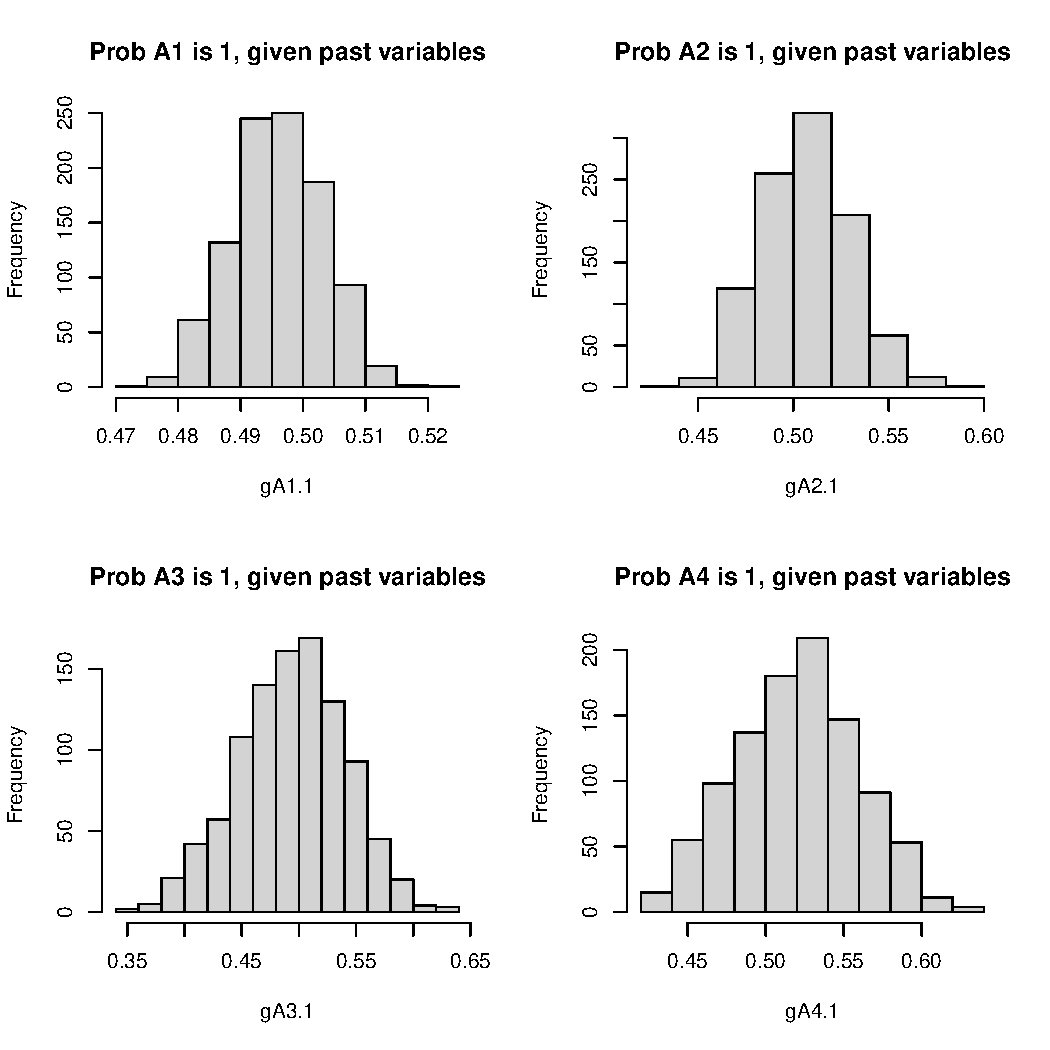
\includegraphics[width=.4\textwidth]{g1Hist2.pdf}
\caption{Plot histograms of $g_n(A(t) = 1|\bar{L}(t), \bar{A}(t-1))$.}
\label{Fig:g1Hist2}
\end{center}
\end{myfigure}

Here, we see that the probabilities of receiving the treatment at each timepoint for all students are around 0.5, and thus far from 0 and 1.
%, especially for the last 3 timepoints. This will likely translate into extreme weights and thus high variability of our estimators.

\begin{Schunk}
\begin{Sinput}
> # predicted probability of the observed treatment (getting 8 or more hrs of sleep) 
> # at time t, given observed history
> # g(A(t)|Lbar(t), Abar(t-1)) = P(A(t)|Lbar(t), Abar(t-1))
> #create empty vectors
> gA1 = gA2 = gA3 = gA4 = rep(NA, length = n)
\end{Sinput}
\end{Schunk}
\begin{Schunk}
\begin{Sinput}
> # for students who got 8 hours of sleep at time 1: 
> # gA1 = P(A(1) = 1|L(1))
> # for students who got less than 8 hours of sleep at time 1:
> # gA1 = P(A(1) = 0|L(1))
> gA1 = (ObsData2$A1 == 1) * gA1.1 + (ObsData2$A1 == 0) * (1 - gA1.1)
> # equivalently
> gA1 = ifelse(ObsData2$A1 == 1, gA1.1, 1-gA1.1)
\end{Sinput}
\end{Schunk}
\begin{Schunk}
\begin{Sinput}
> # repeat for time 2, 3, and 4
> gA2 = (ObsData2$A2 == 1) * gA2.1 + (ObsData2$A2 == 0) * (1 - gA2.1)
> gA3 = (ObsData2$A3 == 1) * gA3.1 + (ObsData2$A3 == 0) * (1 - gA3.1)
> gA4 = (ObsData2$A4 == 1) * gA4.1 + (ObsData2$A4 == 0) * (1 - gA4.1)
\end{Sinput}
\end{Schunk}
\begin{Schunk}
\begin{Sinput}
> # look at the distribution of predicted probabilities 
> # use summary statistics and histograms
> summary(gA1)
\end{Sinput}
\begin{Soutput}
   Min. 1st Qu.  Median    Mean 3rd Qu.    Max. 
 0.4793  0.4943  0.5002  0.5001  0.5058  0.5282 
\end{Soutput}
\begin{Sinput}
> summary(gA2)
\end{Sinput}
\begin{Soutput}
   Min. 1st Qu.  Median    Mean 3rd Qu.    Max. 
 0.4222  0.4849  0.5005  0.5012  0.5177  0.5821 
\end{Soutput}
\begin{Sinput}
> summary(gA3)
\end{Sinput}
\begin{Soutput}
   Min. 1st Qu.  Median    Mean 3rd Qu.    Max. 
 0.3642  0.4742  0.5040  0.5044  0.5374  0.6456 
\end{Soutput}
\begin{Sinput}
> summary(gA4)
\end{Sinput}
\begin{Soutput}
   Min. 1st Qu.  Median    Mean 3rd Qu.    Max. 
 0.3776  0.4716  0.5041  0.5039  0.5344  0.6359 
\end{Soutput}
\begin{Sinput}
> hist(gA1, main = "Prob A1 is observed, given past variables")
> hist(gA2, main = "Prob A2 is observed, given past variables")
> hist(gA3, main = "Prob A3 is observed, given past variables")
> hist(gA4, main = "Prob A4 is observed, given past variables")
\end{Sinput}
\end{Schunk}
\begin{myfigure}
\begin{center}
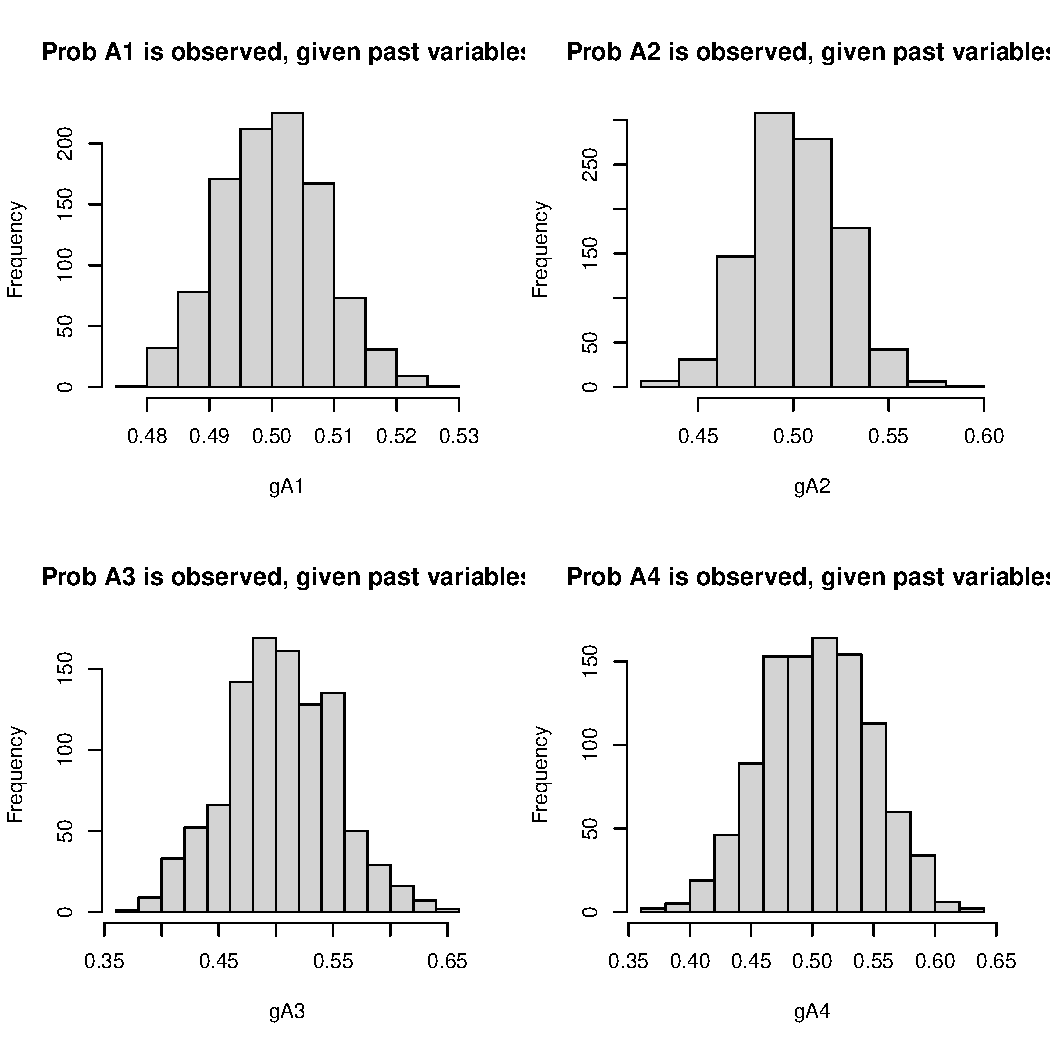
\includegraphics[width=.4\textwidth]{gHist2.pdf}
\caption{Plot histograms of $g_n(A(t)|\bar{L}(t), \bar{A}(t-1))$. }
\label{Fig:gHist2}
\end{center}
\end{myfigure}

Most of the $g_n$ are distributed around 0.51, which does not point to ``near" positivity violations.

IPTW is very sensitive to positivity violations. Based on the summary statistics and histograms, the distributions of $g(A(t)|\bar{L}(t), \bar{A}(t-1))$  show that most covariate/treatment history combinations have a good amount of variability in the exposure at that time point (sleep status at time t).
\begin{Schunk}
\begin{Sinput}
> # indicator variables to identify students with abar(4) = 1 
> # (more than 8 hours of sleep every night) 
> # and abar(4) = 0 
> # (less than 8 hours of sleep every night)
> I1111 = ObsData2$A1 == 1 & ObsData2$A2 == 1 & ObsData2$A3 == 1 & ObsData2$A4 == 1
> I0000 = ObsData2$A1 == 0 & ObsData2$A2 == 0 & ObsData2$A3 == 0 & ObsData2$A4 == 0
\end{Sinput}
\end{Schunk}
\begin{Schunk}
\begin{Sinput}
> # each subject gets a weight inverse to the product of the predicted probabilities
> w = 1/(gA1 * gA2 * gA3 * gA4)
\end{Sinput}
\end{Schunk}
\begin{Schunk}
\begin{Sinput}
> # look at the distribution of the weights
> summary(w)
\end{Sinput}
\begin{Soutput}
   Min. 1st Qu.  Median    Mean 3rd Qu.    Max. 
  8.377  14.524  15.781  16.000  17.159  27.134 
\end{Soutput}
\begin{Sinput}
> hist(w, main = "Distribution of weights")
\end{Sinput}
\end{Schunk}
\begin{myfigure}
\begin{center}
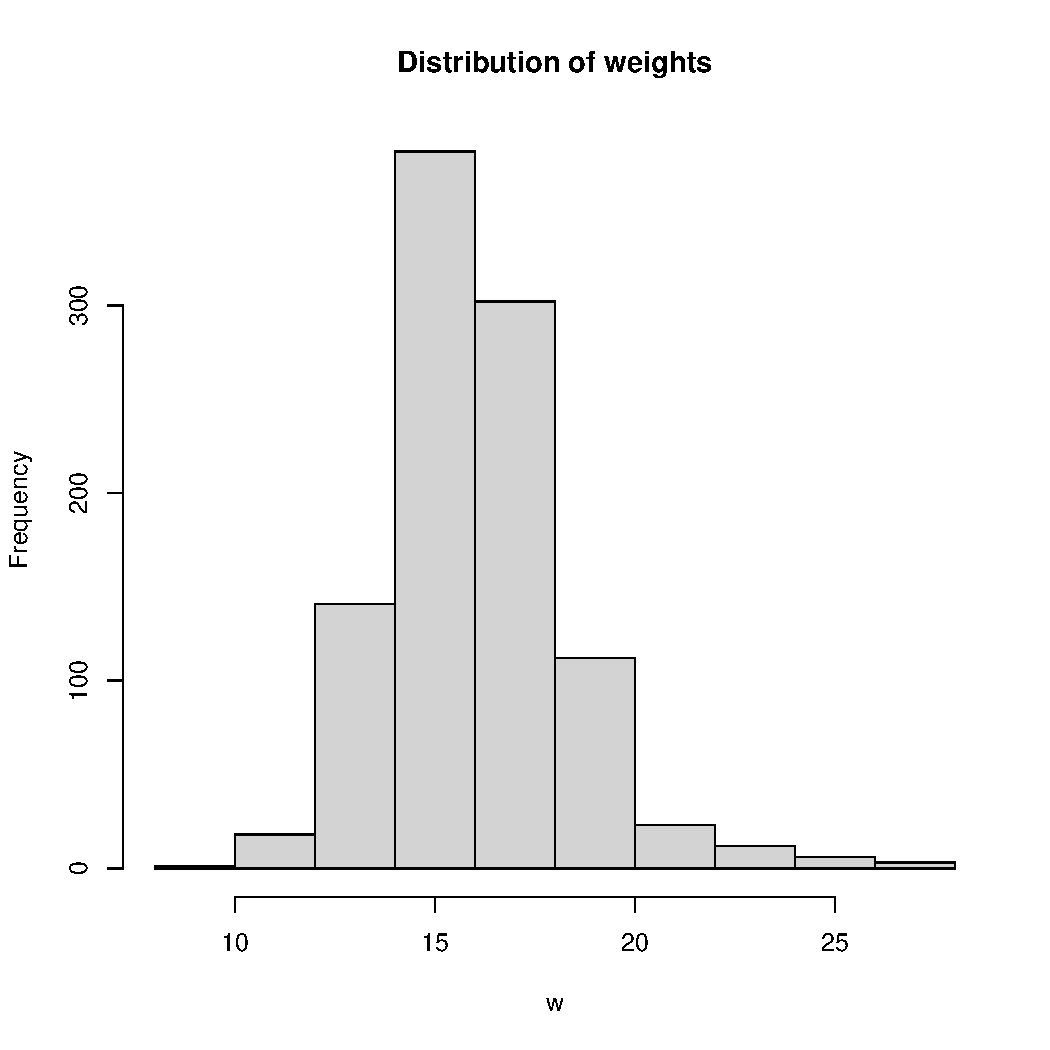
\includegraphics[width=.4\textwidth]{wHist2.pdf}
\caption{Distribution of weights.}
\label{Fig:wHist2}
\end{center}
\end{myfigure}


\begin{Schunk}
\begin{Sinput}
> # look at the distribution of the weights for people 
> # who got 8 or more hours of sleep for entire study
> summary(w[I1111])
\end{Sinput}
\begin{Soutput}
   Min. 1st Qu.  Median    Mean 3rd Qu.    Max. 
  13.06   15.10   15.90   15.87   16.69   18.39 
\end{Soutput}
\begin{Sinput}
> hist(w[I1111], main = "Distribution of weights 
+      for people with treatment history = 1")
\end{Sinput}
\end{Schunk}
\begin{myfigure}
\begin{center}
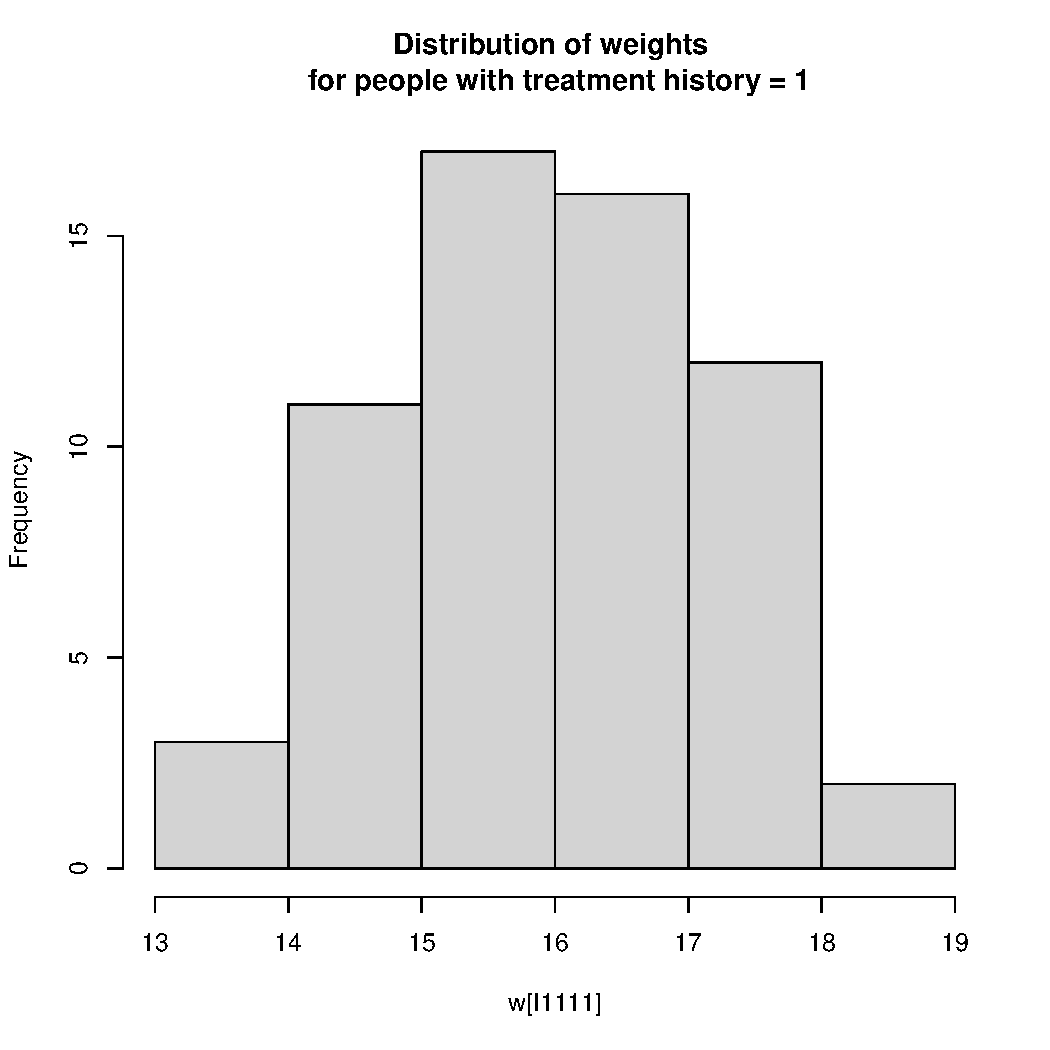
\includegraphics[width=.4\textwidth]{w1111Hist2.pdf}
\caption{Distribution of weights for subjects who receive treatment at all timepoints.}
\label{Fig:w1111Hist2}
\end{center}
\end{myfigure}

Although the conditional probabilities of treatment at each individual timepoint did not look concerning (i.e., most were around 0.5), because we have several time points, the denominator of the weights will be a product of several probabilities, which translates to high weights. This is something that's reflected in the distribution of the estimated weights: the summary statistics show that at least one student who got more than 8 hours of sleep will be upweighted by 18.3913. 

\begin{Schunk}
\begin{Sinput}
> # look at the distribution of the weights 
> # for people who got less than 8 hours of sleep for entire study
> summary(w[I0000])
\end{Sinput}
\begin{Soutput}
   Min. 1st Qu.  Median    Mean 3rd Qu.    Max. 
  14.03   15.69   16.62   16.48   17.19   18.97 
\end{Soutput}
\begin{Sinput}
> hist(w[I0000], 
+      main = "Distribution of weights \n for people with treatment history = 0")
\end{Sinput}
\end{Schunk}
\begin{myfigure}
\begin{center}
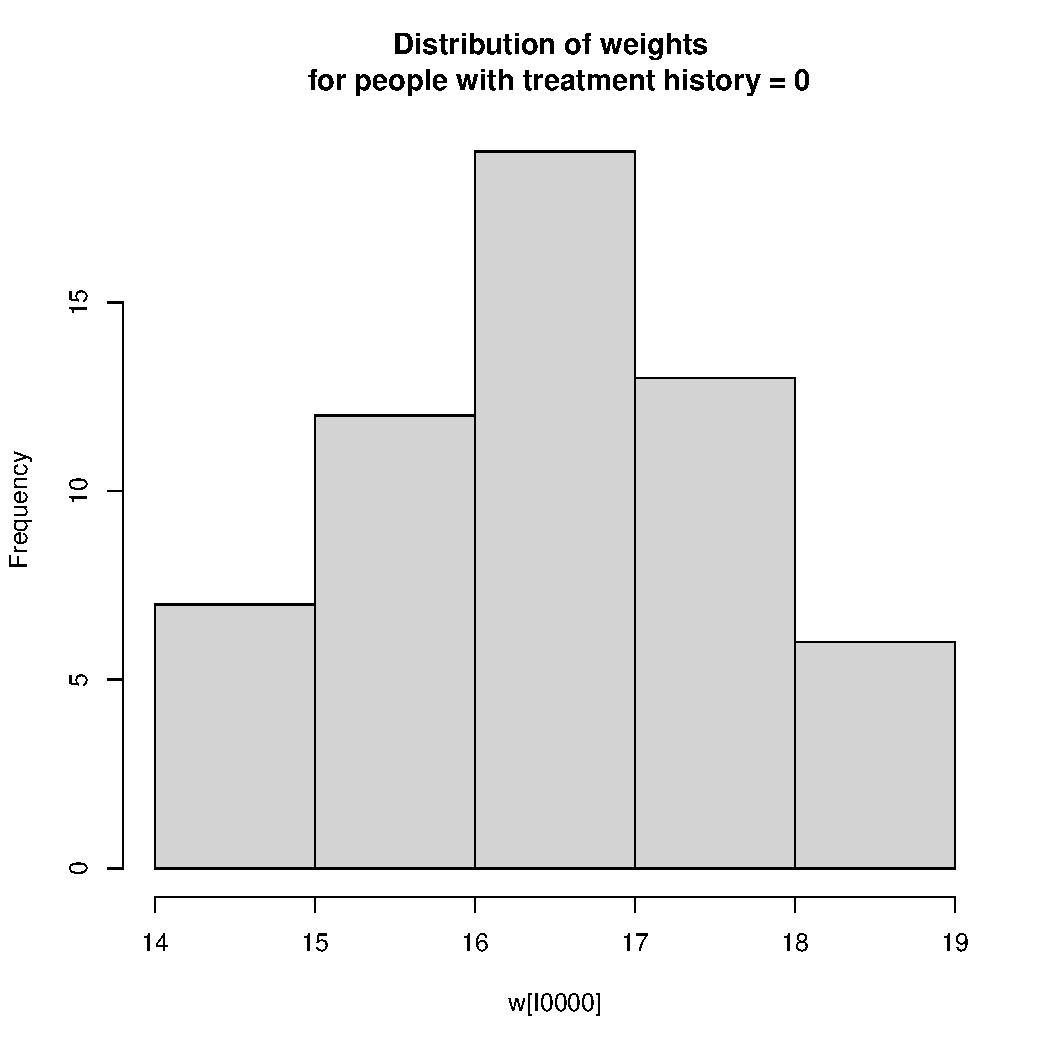
\includegraphics[width=.4\textwidth]{w0000Hist2.pdf}
\caption{Distribution of weights for subjects who do not receive treatment at all timepoints.}
\label{Fig:w0000Hist2}
\end{center}
\end{myfigure}

And at least one student who did not get more than 8 hours of sleep will be upweighted by 18.9664.


\begin{Schunk}
\begin{Sinput}
> # point estimate: weighted empirical mean outcome for students with abar(4) = 1 
> # minus the weighted empirical mean for students with abar(4) = 0 
> IPTW = mean(ObsData2$Y * I1111 * w) - mean(ObsData2$Y * I0000 * w)
> IPTW
\end{Sinput}
\begin{Soutput}
[1] 15.56433
\end{Soutput}
\end{Schunk}


\begin{Schunk}
\begin{Sinput}
> # modified Horvitz-Thompson estimator
> IPTW.HT = mean(ObsData2$Y * I1111 * w)/mean(I1111 * w) - 
+   mean(ObsData2$Y * I0000 * w)/mean(I0000 * w)
> IPTW.HT
\end{Sinput}
\begin{Soutput}
[1] 14.38082
\end{Soutput}
\end{Schunk}

The standard IPTW estimate was 15.5643. The Horvitz-Thompson estimate was 14.3808. These are estimates of the average difference in expected test score among students who got 8 or more hours of sleep for all 4 nights versus students who got less than 8 hours of sleep for all 4 nights, weighted by student's estimated treatment mechanism.

Recall that $\Psi^F(P_{U,X})$, the true expected difference in counterfactual test scores, is 13.62. In the next section, we'll measure these estimators' performances against the truth.

\begin{Schunk}
\begin{Sinput}
> # calculate the observed cumulative abar(4) for each subject
> sum.a = rowSums(ObsData2[c("A1", "A2", "A3", "A4")])
\end{Sinput}
\end{Schunk}
\begin{Schunk}
\begin{Sinput}
> # estimate the parameters of the MSM with IPTW weights
> IPTW.MSM = glm(Y ~ sum.a, data = ObsData2, weights = w)
> IPTW.MSM.coef = IPTW.MSM$coefficients[["sum.a"]] # extract the Beta1 coefficient
> IPTW.MSM.coef
\end{Sinput}
\begin{Soutput}
[1] 3.343084
\end{Soutput}
\end{Schunk}
The estimated parameters of the MSM are 
\begin{align*}
m(\bar{a}|\beta) & = \hat{\beta}_0 + \hat{\beta_1}\sum_{t=1}^4a(t) \\
& = 57.85 + 3.34\sum_{t=1}^4a(t)
\end{align*}

Under the necessary causal assumptions, and if we assume the MSM is correct, we can interpret $\hat{\beta}_1$ as follows: for one more night of sleep, the average test score increases by 3.34. Recall that the true value of $\beta_1$ using projection function $g^*(\bar{A}) = 1$ was 3.4.

\vspace{4mm}
\textit{Bonus!} Calculating the parameters of an MSM using \textit{stabilized} IPTW weights.
\begin{Schunk}
\begin{Sinput}
> # create every permutation of abar(4)
> abar = expand.grid(c(0,1), c(0,1), c(0,1), c(0,1))
\end{Sinput}
\end{Schunk}
\begin{Schunk}
\begin{Sinput}
> # create a new vector for the marginal probability of each permutation of abar(4)
> # in other words, g(abar(4))
> g.abar = rep(NA, n)
\end{Sinput}
\end{Schunk}
\begin{Schunk}
\begin{Sinput}
> # for each possible permutation of abar(4), find the marginal probability. 
> # assign that probability to each subject who has that observed abar(4).
> for(i in 1:16){
+   
+   marg.prob = mean(ObsData2$A1 == abar[i,1] & 
+                      ObsData2$A2 == abar[i,2] & 
+                      ObsData2$A3 == abar[i,3] & 
+                      ObsData2$A4 == abar[i,4]) # marginal probability
+   
+   g.abar[ObsData2$A1 == abar[i,1] & 
+            ObsData2$A2 == abar[i,2] & 
+            ObsData2$A3 == abar[i,3] & 
+            ObsData2$A4 == abar[i,4]] = marg.prob # assign to subject in vector g.abar
+   
+ }
\end{Sinput}
\end{Schunk}
\begin{Schunk}
\begin{Sinput}
> # multiply the original weights by the numerator to obtain the the stabilized weights
> sw = g.abar*w
\end{Sinput}
\end{Schunk}
\begin{Schunk}
\begin{Sinput}
> summary(sw)
\end{Sinput}
\begin{Soutput}
   Min. 1st Qu.  Median    Mean 3rd Qu.    Max. 
 0.5278  0.9165  0.9968  1.0032  1.0780  1.5920 
\end{Soutput}
\begin{Sinput}
> hist(sw, main = "Distribution of stabilized weights")
\end{Sinput}
\end{Schunk}
After stabilization, the weights are less variable and extreme.
\begin{Schunk}
\begin{Sinput}
> # estimate the parameters of the MSM with IPTW stabilized weights
> IPTW.MSM.stab = glm(Y ~ sum.a, data = ObsData2, weights = sw)
> IPTW.MSM.stab.coef = IPTW.MSM.stab$coefficients[[2]] # extract the Beta1 coefficient
> IPTW.MSM.stab.coef
\end{Sinput}
\begin{Soutput}
[1] 3.315394
\end{Soutput}
\end{Schunk}

The estimated parameters of the MSM using IPTW with stabilized weights are 
\begin{align*}
m(\bar{a}|\beta) & = \hat{\beta}_0 + \hat{\beta_1}\sum_{t=1}^4a(t) \\
& = 57.85 + 3.32\sum_{t=1}^4a(t)
\end{align*}

Recall that the $\beta_1$ on our true causal curve using projection function $g^*(\bar{A}) = g(\bar{A}(4))$ is equal to 3.4.
\end{solution}

\item \textbf{Estimator performance metrics:}

\begin{enumerate}
\item Set the number of iterations \texttt{B} to 5 (to start)
\item Create a matrix \texttt{estimates\_data2} with \texttt{B} rows and 2 columns. Name the columns of the matrix \texttt{IPTW, IPTW.HT}. \\
\textit{Note:} If you calculated the MSM parameters without and with stabilized weights (i.e., the bonus question in the previous section), create 4 columns in your matrix instead of 2, and name the $3^{rd}$ and $4^{th}$ columns \texttt{IPTW.MSM.coef} and \texttt{IPTW.MSM.stab.coef}, respectively.
\item Within a for loop from \texttt{b} to \texttt{1:B}, do the following:
\begin{enumerate}
\item Redraw $n$ copies of the data using the \texttt{generate\_data2()} function you loaded earlier. 
\item Copy and paste code from the previous steps (making sure to remove any plots!) to generate 2 new IPTW estimates (4 IPTW estimates if you calculated the MSM parameters) using the redrawn data in the previous step. Specifically: 
\begin{enumerate}
\item[1.] Estimate the treatment mechanism
\item[2.] Predict the conditional probability of having the exposure
\item[3.] Predict the probability of having the observed exposure
\item[4.] Create weights
\item[5.] Generate the standard and Horvitz-Thompson IPTW estimates
\item[6.] Generate coefficient estimates of the MSM (Fall 2020 -- not required)
\end{enumerate}
\item Save the estimates in the $b^{th}$ row of the \texttt{estimates\_data2} matrix.
\begin{Schunk}
\begin{Sinput}
> estimates_data2[b,] = c(IPTW, IPTW.HT)
> estimates_data2[b,] = c(IPTW, IPTW.HT, IPTW.MSM.coef, IPTW.MSM.stab.coef) # with MSM
\end{Sinput}
\end{Schunk}
\textit{Note:} again, if you estimated a stabilized MSM, add \texttt{IPTW.MSM.stab.coef} to the end of this vector.
\end{enumerate}
\item When you are confident that your code is working, set the seed to 252 and increase the number of iterations \texttt{B = 500} and rerun your code. 
\item For each estimator, estimate the:
\begin{itemize}
\item[-] Bias. \textit{Hint:} use the \texttt{colMeans()} function.
\item[-] Variance. \textit{Hint:} use the \texttt{var()} function on the estimates to get the covariance matrix, and take the diagonal of that matrix using the \texttt{diag()} function to get each estimator's variance.
\item[-] MSE. \textit{Hint:} use the \texttt{colMeans()} function.
\end{itemize}
\end{enumerate}
\end{enumerate}

\begin{solution}
\begin{Schunk}
\begin{Sinput}
> ### IPTW estimator performance metrics - Data 2 ###
> # set seed
> set.seed(252)
> # number of iterations
> B = 500
\end{Sinput}
\end{Schunk}
\begin{Schunk}
\begin{Sinput}
> # matrix to store IPTW estimates
> estimates_data2 = matrix(NA, nrow = B, ncol = 4)
> # column names for matrix
> colnames(estimates_data2) = c("IPTW", "IPTW.HT", "IPTW.MSM.coef", "IPTW.MSM.stab.coef")
\end{Sinput}
\end{Schunk}
\begin{Schunk}
\begin{Sinput}
> # for loop that creates many iterations of ObsData2 and implements above IPTW estimates
> for(b in 1:B) {
+   
+   # redraw the data
+   ObsData2 = generate_data2(n)
+   
+   # estimate treatment mechanisms
+   gA1.reg = glm(A1 ~ L1, family = "binomial", data = ObsData2)
+   gA2.reg = glm(A2 ~ L1 + A1 + L2, family = "binomial", data = ObsData2)
+   gA3.reg = glm(A3 ~ L1 + A1 + L2 + A2 + L3, family = "binomial", data = ObsData2)
+   gA4.reg = glm(A4 ~ L1 + A1 + L2 + A2 + L3 + A3 + L4, family = "binomial", data = ObsData2)
+   
+   # predicted probability of having exposure, given history
+   gA1.1 = predict(gA1.reg, type = "response")
+   gA2.1 = predict(gA2.reg, type = "response")
+   gA3.1 = predict(gA3.reg, type = "response")
+   gA4.1 = predict(gA4.reg, type = "response")
+   
+   # predicted probability of observed exposure, given history
+   gA1 = (ObsData2$A1 == 1) * gA1.1 + (ObsData2$A1 == 0) * (1 - gA1.1)
+   gA2 = (ObsData2$A2 == 1) * gA2.1 + (ObsData2$A2 == 0) * (1 - gA2.1)
+   gA3 = (ObsData2$A3 == 1) * gA3.1 + (ObsData2$A3 == 0) * (1 - gA3.1)
+   gA4 = (ObsData2$A4 == 1) * gA4.1 + (ObsData2$A4 == 0) * (1 - gA4.1)
+   
+   # weight = inverse of predicted probability
+   w = 1/(gA1 * gA2 * gA3 * gA4)
+   
+   # indicators of observed abar(4) = 1 and abar(4) = 0
+   I1111 = ObsData2$A1 == 1 & ObsData2$A2 == 1 & ObsData2$A3 == 1 & ObsData2$A4 == 1
+   I0000 = ObsData2$A1 == 0 & ObsData2$A2 == 0 & ObsData2$A3 == 0 & ObsData2$A4 == 0
+   
+   # IPTW estimate for g-comp estimand 
+   IPTW = mean(ObsData2$Y * I1111 * w) - mean(ObsData2$Y * I0000 * w)
+   # Horvitz-Thompson IPTW estimate for g-comp estimand 
+   IPTW.HT = mean(ObsData2$Y * I1111 * w)/mean(I1111 * w) - 
+     mean(ObsData2$Y * I0000 * w)/mean(I0000 * w)
+   
+   # get cumulative abars
+   ObsData2$sum.a = rowSums(ObsData2[c("A1", "A2", "A3", "A4")])
+   
+   # MSM and coefficient (unstabilized)
+   IPTW.MSM = glm(Y ~ sum.a, data = ObsData2, weights = w)
+   IPTW.MSM.coef = IPTW.MSM$coefficients[[2]]
+   
+   # create stabilized weights
+   abar = expand.grid(c(0,1), c(0,1), c(0,1), c(0,1))
+   g.abar = rep(NA, n)
+   for(i in 1:16){
+     marg.prob = mean(ObsData2$A1 == abar[i,1] & 
+                        ObsData2$A2 == abar[i,2] & 
+                        ObsData2$A3 == abar[i,3] & 
+                        ObsData2$A4 == abar[i,4]) 
+     g.abar[ObsData2$A1 == abar[i,1] & 
+              ObsData2$A2 == abar[i,2] & 
+              ObsData2$A3 == abar[i,3] & 
+              ObsData2$A4 == abar[i,4]] = marg.prob 
+   }
+   sw = g.abar*w # stabilized weights
+   
+   # MSM and coefficient (stabilized)
+   IPTW.MSM.stab = glm(Y ~ sum.a, data = ObsData2, weights = sw)
+   IPTW.MSM.stab.coef = IPTW.MSM.stab$coefficients[[2]]
+   
+   # store estimates in matrix
+   estimates_data2[b,] = c(IPTW, IPTW.HT, IPTW.MSM.coef, IPTW.MSM.stab.coef)
+   
+ }
\end{Sinput}
\end{Schunk}
\begin{Schunk}
\begin{Sinput}
> # Bias
> # bias for IPTW and IPTW HT
> colMeans(estimates_data2[,1:2] - Psi.F2)
\end{Sinput}
\begin{Soutput}
       IPTW     IPTW.HT 
-0.25334760 -0.07368556 
\end{Soutput}
\begin{Sinput}
> # bias for betas on stabilized and unstabilized MSM
> mean(estimates_data2[,3] - TrueMSMbeta1)
\end{Sinput}
\begin{Soutput}
[1] -0.007173814
\end{Soutput}
\begin{Sinput}
> mean(estimates_data2[,4] - TrueMSMbeta1_wts)
\end{Sinput}
\begin{Soutput}
[1] -0.01123337
\end{Soutput}
\end{Schunk}
\begin{Schunk}
\begin{Sinput}
> # Variance
> diag(var(estimates_data2))
\end{Sinput}
\begin{Soutput}
              IPTW            IPTW.HT      IPTW.MSM.coef IPTW.MSM.stab.coef 
       63.27533483         1.29722683         0.01553514         0.01705657 
\end{Soutput}
\end{Schunk}
\begin{Schunk}
\begin{Sinput}
> # MSE
> # MSE for IPTW and IPTW HT
> colMeans((estimates_data2[,1:2] - Psi.F2)^2)
\end{Sinput}
\begin{Soutput}
     IPTW   IPTW.HT 
63.212969  1.300062 
\end{Soutput}
\begin{Sinput}
> # MSE for beta1 on stabilized and unstabilized MSM
> mean((estimates_data2[,3] - TrueMSMbeta1)^2)
\end{Sinput}
\begin{Soutput}
[1] 0.01555553
\end{Soutput}
\begin{Sinput}
> mean((estimates_data2[,4] - TrueMSMbeta1_wts)^2)
\end{Sinput}
\begin{Soutput}
[1] 0.01714865
\end{Soutput}
\end{Schunk}

\end{solution}


\pagebreak
\section{For Your Project: IPTW Estimation}

Think through the following questions and apply them to the dataset you will use for your final project.

\begin{enumerate}
\item \textbf{Treatment/censoring mechanism}
\begin{enumerate}
\item What are the necessary parts of your $P_0$ that you need for IPTW implementation?
\item Estimate these parts using parametric regressions or SuperLearner. What do the predicted probabilities of treatment/censoring look like? Any cause for concern?
\item Create weights (and stabilized weights if working with an MSM) based on these estimates. What do they look like? Any cause for concern? Was there something you could see in the distribution of the weights that you couldn't spot by just looking at the predicted probabilities in the previous step?
\end{enumerate}
\item \textbf{Implement IPTW}
\begin{enumerate}
\item Implement standard IPTW and modified Horvitz-Thompson IPTW for treatment-specific mean causal questions. Depending on whether you are using an MSM to define your target parameter, use a weighted regression with stablized and unstabilized IPTW weights for evaluating parameters of an MSM.
\item Interpret the estimates generated in the previous question in the context of your study.
\end{enumerate}
\item \textbf{Performance of IPTW}
\begin{enumerate}
\item Evaluate the bias, variance, and MSE of your IPTW estimator by comparing it against the ``true" causal estimand you generated in \texttt{R} Lab 2.
\end{enumerate}
\end{enumerate}

\pagebreak

\section{Feedback}

Please attach responses to these questions to your lab. Thank you in advance!

\begin{enumerate}
\item Did you catch any errors in this lab? If so, where?
\item What did you learn in this lab?
\item Do you think that this lab met the goals listed at the beginning? 
\item What else would you have liked to review? What would have helped your understanding?
\item Any other feedback?
\end{enumerate}

\end{document}


